\chapter{Usmjereni grafovi}

U ovom poglavlju usredotočit ćemo se na dvije klase usmjerenih grafova:
\begin{itemize}
\item \key{Aciklički grafovi}:
U grafu nema ciklusa,
pa ne postoji put od bilo kojeg čvora do njega samoga\footnote{Usmjereni aciklički
grafovi se ponekad nazivaju DAG-ovi.}.
\item \key{Grafovi sljedbenika}:
Izlazni stupanj svakog čvora je 1,
pa svaki čvor ima jedinstvenog sljedbenika.
\end{itemize}
Pokazuje se da u oba slučaja
možemo osmisliti efikasne algoritme koji se temelje
na posebnim svojstvima tih grafova.

\section{Topološko sortiranje}

\index{topološko sortiranje}
\index{ciklus}

\key{Topološko sortiranje} je uređaj
čvorova usmjerenog grafa
takav da ako postoji put od čvora $a$ do čvora $b$,
tada čvor $a$ dolazi prije čvora $b$ u tom uređaju.
Na primjer, za graf
\begin{center}
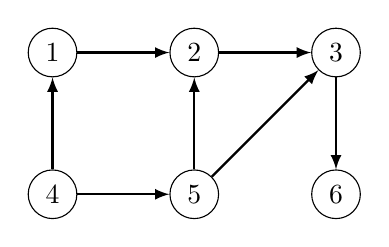
\begin{tikzpicture}[scale=0.9]
\node[draw, circle] (1) at (1,5) {$1$};
\node[draw, circle] (2) at (3,5) {$2$};
\node[draw, circle] (3) at (5,5) {$3$};
\node[draw, circle] (4) at (1,3) {$4$};
\node[draw, circle] (5) at (3,3) {$5$};
\node[draw, circle] (6) at (5,3) {$6$};

\path[draw,thick,->,>=latex] (1) -- (2);
\path[draw,thick,->,>=latex] (2) -- (3);
\path[draw,thick,->,>=latex] (4) -- (1);
\path[draw,thick,->,>=latex] (4) -- (5);
\path[draw,thick,->,>=latex] (5) -- (2);
\path[draw,thick,->,>=latex] (5) -- (3);
\path[draw,thick,->,>=latex] (3) -- (6);
\end{tikzpicture}
\end{center}
jedno topološko sortiranje je
$[4,1,5,2,3,6]$:
\begin{center}
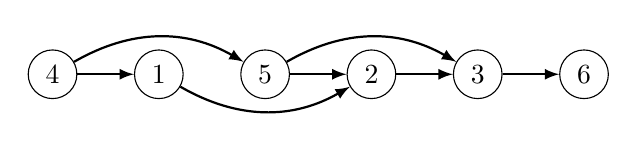
\begin{tikzpicture}[scale=0.9]
\node[draw, circle] (1) at (-6,0) {$1$};
\node[draw, circle] (2) at (-3,0) {$2$};
\node[draw, circle] (3) at (-1.5,0) {$3$};
\node[draw, circle] (4) at (-7.5,0) {$4$};
\node[draw, circle] (5) at (-4.5,0) {$5$};
\node[draw, circle] (6) at (-0,0) {$6$};

\path[draw,thick,->,>=latex] (1) edge [bend right=30] (2);
\path[draw,thick,->,>=latex] (2) -- (3);
\path[draw,thick,->,>=latex] (4) -- (1);
\path[draw,thick,->,>=latex] (4) edge [bend left=30] (5);
\path[draw,thick,->,>=latex] (5) -- (2);
\path[draw,thick,->,>=latex] (5) edge [bend left=30]  (3);
\path[draw,thick,->,>=latex] (3) -- (6);
\end{tikzpicture}
\end{center}

Acikliči graf uvijek ima topološko sortiranje.
Međutim, ako graf sadrži ciklus,
nije moguće oblikovati topološko sortiranje,
jer nijedan čvor ciklusa ne može doći
prije ostalih čvorova ciklusa u tom uređaju.
Pokazuje se da se pretraživanje u dubinu može upotrijebiti
i za provjeru sadrži li usmjereni graf ciklus
i, ako ne sadrži ciklus, za konstrukciju topološkog sortiranja.

\subsubsection{Algoritam}

Ideja je proći kroz čvorove grafa
i uvijek započeti pretraživanje u dubinu u trenutnom čvoru
ako on još nije obrađen.
Tijekom pretraživanja čvorovi imaju tri moguća stanja:

\begin{itemize}
\item stanje 0: čvor nije obrađen (bijelo)
\item stanje 1: čvor je u obradi (svjetlosivo)
\item stanje 2: čvor je obrađen (tamnosivo)
\end{itemize}

Na početku je stanje svakog čvora 0.
Kada pretraživanje prvi put dođe do nekog čvora,
njegovo stanje postaje 1.
Konačno, nakon što su svi sljedbenici čvora
obrađeni, njegovo stanje postaje 2.

Ako graf sadrži ciklus, to ćemo otkriti
tijekom pretraživanja, jer ćemo prije ili poslije
doći do čvora čije je stanje 1.
U tom slučaju nije moguće konstruirati topološko sortiranje.

Ako graf ne sadrži ciklus, možemo konstruirati
topološko sortiranje tako da
svaki čvor dodamo u listu kada stanje čvora postane 2.
Ta lista u obrnutom redoslijedu je topološko sortiranje.

\subsubsection{Primjer 1}

U primjeru grafa pretraživanje najprije ide
od čvora 1 do čvora 6:

\begin{center}
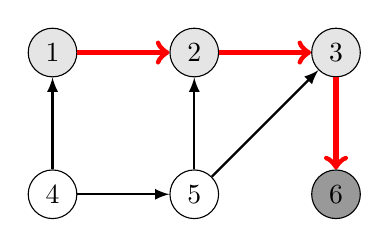
\begin{tikzpicture}[scale=0.9]
\node[draw, circle,fill=gray!20] (1) at (1,5) {$1$};
\node[draw, circle,fill=gray!20] (2) at (3,5) {$2$};
\node[draw, circle,fill=gray!20] (3) at (5,5) {$3$};
\node[draw, circle] (4) at (1,3) {$4$};
\node[draw, circle] (5) at (3,3) {$5$};
\node[draw, circle,fill=gray!80] (6) at (5,3) {$6$};

\path[draw,thick,->,>=latex] (4) -- (1);
\path[draw,thick,->,>=latex] (4) -- (5);
\path[draw,thick,->,>=latex] (5) -- (2);
\path[draw,thick,->,>=latex] (5) -- (3);
%\path[draw,thick,->,>=latex] (3) -- (6);

\path[draw=red,thick,->,line width=2pt] (1) -- (2);
\path[draw=red,thick,->,line width=2pt] (2) -- (3);
\path[draw=red,thick,->,line width=2pt] (3) -- (6);
\end{tikzpicture}
\end{center}

Sada je čvor 6 obrađen, pa se dodaje u listu.
Nakon toga se u listu dodaju i čvorovi 3, 2 i 1:

\begin{center}
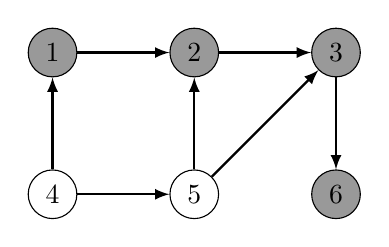
\begin{tikzpicture}[scale=0.9]
\node[draw, circle,fill=gray!80] (1) at (1,5) {$1$};
\node[draw, circle,fill=gray!80] (2) at (3,5) {$2$};
\node[draw, circle,fill=gray!80] (3) at (5,5) {$3$};
\node[draw, circle] (4) at (1,3) {$4$};
\node[draw, circle] (5) at (3,3) {$5$};
\node[draw, circle,fill=gray!80] (6) at (5,3) {$6$};

\path[draw,thick,->,>=latex] (1) -- (2);
\path[draw,thick,->,>=latex] (2) -- (3);
\path[draw,thick,->,>=latex] (4) -- (1);
\path[draw,thick,->,>=latex] (4) -- (5);
\path[draw,thick,->,>=latex] (5) -- (2);
\path[draw,thick,->,>=latex] (5) -- (3);
\path[draw,thick,->,>=latex] (3) -- (6);
\end{tikzpicture}
\end{center}

U ovom trenutku lista je $[6,3,2,1]$.
Sljedeće pretraživanje počinje u čvoru 4:

\begin{center}
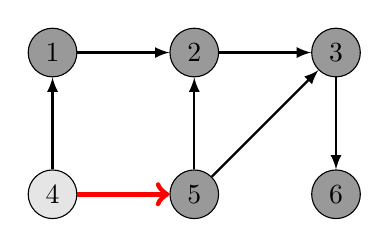
\begin{tikzpicture}[scale=0.9]
\node[draw, circle,fill=gray!80] (1) at (1,5) {$1$};
\node[draw, circle,fill=gray!80] (2) at (3,5) {$2$};
\node[draw, circle,fill=gray!80] (3) at (5,5) {$3$};
\node[draw, circle,fill=gray!20] (4) at (1,3) {$4$};
\node[draw, circle,fill=gray!80] (5) at (3,3) {$5$};
\node[draw, circle,fill=gray!80] (6) at (5,3) {$6$};

\path[draw,thick,->,>=latex] (1) -- (2);
\path[draw,thick,->,>=latex] (2) -- (3);
\path[draw,thick,->,>=latex] (4) -- (1);
%\path[draw,thick,->,>=latex] (4) -- (5);
\path[draw,thick,->,>=latex] (5) -- (2);
\path[draw,thick,->,>=latex] (5) -- (3);
\path[draw,thick,->,>=latex] (3) -- (6);

\path[draw=red,thick,->,line width=2pt] (4) -- (5);
\end{tikzpicture}
\end{center}

Dakle, konačna lista je $[6,3,2,1,5,4]$.
Obradili smo sve čvorove, pa je topološko sortiranje
nađeno.
Topološko sortiranje je obrnuta lista
$[4,5,1,2,3,6]$:

\begin{center}
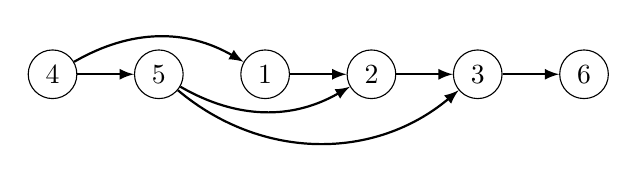
\begin{tikzpicture}[scale=0.9]
\node[draw, circle] (1) at (3,0) {$1$};
\node[draw, circle] (2) at (4.5,0) {$2$};
\node[draw, circle] (3) at (6,0) {$3$};
\node[draw, circle] (4) at (0,0) {$4$};
\node[draw, circle] (5) at (1.5,0) {$5$};
\node[draw, circle] (6) at (7.5,0) {$6$};

\path[draw,thick,->,>=latex] (1) -- (2);
\path[draw,thick,->,>=latex] (2) -- (3);
\path[draw,thick,->,>=latex] (4) edge [bend left=30] (1);
\path[draw,thick,->,>=latex] (4) -- (5);
\path[draw,thick,->,>=latex] (5) edge [bend right=30] (2);
\path[draw,thick,->,>=latex] (5) edge [bend right=40] (3);
\path[draw,thick,->,>=latex] (3) -- (6);
\end{tikzpicture}
\end{center}

Uočimo da topološko sortiranje nije jedinstveno
te da za graf može postojati više topoloških sortiranja.

\subsubsection{Primjer 2}

Razmotrimo sada graf za koji
ne možemo konstruirati topološko sortiranje,
jer graf sadrži ciklus:

\begin{center}
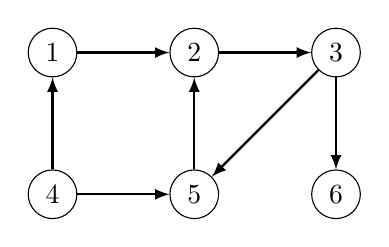
\begin{tikzpicture}[scale=0.9]
\node[draw, circle] (1) at (1,5) {$1$};
\node[draw, circle] (2) at (3,5) {$2$};
\node[draw, circle] (3) at (5,5) {$3$};
\node[draw, circle] (4) at (1,3) {$4$};
\node[draw, circle] (5) at (3,3) {$5$};
\node[draw, circle] (6) at (5,3) {$6$};

\path[draw,thick,->,>=latex] (1) -- (2);
\path[draw,thick,->,>=latex] (2) -- (3);
\path[draw,thick,->,>=latex] (4) -- (1);
\path[draw,thick,->,>=latex] (4) -- (5);
\path[draw,thick,->,>=latex] (5) -- (2);
\path[draw,thick,->,>=latex] (3) -- (5);
\path[draw,thick,->,>=latex] (3) -- (6);
\end{tikzpicture}
\end{center}
Pretraživanje se odvija na sljedeći način:
\begin{center}
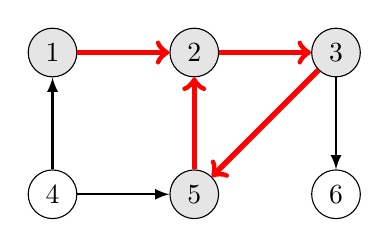
\begin{tikzpicture}[scale=0.9]
\node[draw, circle,fill=gray!20] (1) at (1,5) {$1$};
\node[draw, circle,fill=gray!20] (2) at (3,5) {$2$};
\node[draw, circle,fill=gray!20] (3) at (5,5) {$3$};
\node[draw, circle] (4) at (1,3) {$4$};
\node[draw, circle,fill=gray!20] (5) at (3,3) {$5$};
\node[draw, circle] (6) at (5,3) {$6$};

\path[draw,thick,->,>=latex] (4) -- (1);
\path[draw,thick,->,>=latex] (4) -- (5);
\path[draw,thick,->,>=latex] (3) -- (6);

\path[draw=red,thick,->,line width=2pt] (1) -- (2);
\path[draw=red,thick,->,line width=2pt] (2) -- (3);
\path[draw=red,thick,->,line width=2pt] (3) -- (5);
\path[draw=red,thick,->,line width=2pt] (5) -- (2);
\end{tikzpicture}
\end{center}
Pretraživanje dolazi do čvora 2 čije je stanje 1,
što znači da graf sadrži ciklus.
U ovom primjeru postoji ciklus
$2 \rightarrow 3 \rightarrow 5 \rightarrow 2$.

\section{Dinamičko programiranje}

Ako je usmjereni graf aciklički,
na njega se može primijeniti dinamičko programiranje.
Na primjer, možemo efikasno riješiti sljedeće
zadatke o putovima od početnog čvora
do završnog čvora:

\begin{itemize}
\item koliko različitih putova postoji?
\item koji je najkraći/najdulji put?
\item koji je najmanji/najveći broj bridova u putu?
\item koji se čvorovi sigurno pojavljuju u svakom putu?
\end{itemize}

\subsubsection{Prebrojavanje putova}

Kao primjer, izračunajmo broj putova
od čvora 1 do čvora 6 u sljedećem grafu:

\begin{center}
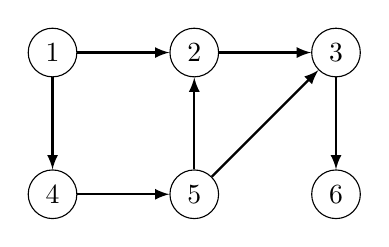
\begin{tikzpicture}[scale=0.9]
\node[draw, circle] (1) at (1,5) {$1$};
\node[draw, circle] (2) at (3,5) {$2$};
\node[draw, circle] (3) at (5,5) {$3$};
\node[draw, circle] (4) at (1,3) {$4$};
\node[draw, circle] (5) at (3,3) {$5$};
\node[draw, circle] (6) at (5,3) {$6$};

\path[draw,thick,->,>=latex] (1) -- (2);
\path[draw,thick,->,>=latex] (2) -- (3);
\path[draw,thick,->,>=latex] (1) -- (4);
\path[draw,thick,->,>=latex] (4) -- (5);
\path[draw,thick,->,>=latex] (5) -- (2);
\path[draw,thick,->,>=latex] (5) -- (3);
\path[draw,thick,->,>=latex] (3) -- (6);
\end{tikzpicture}
\end{center}
Ukupno postoje tri takva puta:
\begin{itemize}
\item $1 \rightarrow 2 \rightarrow 3 \rightarrow 6$
\item $1 \rightarrow 4 \rightarrow 5 \rightarrow 2 \rightarrow 3 \rightarrow 6$
\item $1 \rightarrow 4 \rightarrow 5 \rightarrow 3 \rightarrow 6$
\end{itemize}

Označimo s $\texttt{paths}(x)$ broj putova od
čvora 1 do čvora $x$.
Kao bazni slučaj imamo $\texttt{paths}(1)=1$.
Zatim, za izračun ostalih vrijednosti $\texttt{paths}(x)$,
možemo koristiti rekurziju
\[\texttt{paths}(x) = \texttt{paths}(a_1)+\texttt{paths}(a_2)+\cdots+\texttt{paths}(a_k)\]
gdje su $a_1,a_2,\ldots,a_k$ čvorovi iz kojih postoji
brid do $x$.
Budući da je graf aciklički, vrijednosti $\texttt{paths}(x)$
mogu se izračunati u redoslijedu topološkog sortiranja.
Topološko sortiranje za gornji graf izgleda ovako:
\begin{center}
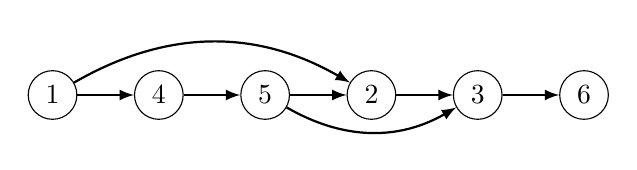
\begin{tikzpicture}[scale=0.9]
\node[draw, circle] (1) at (0,0) {$1$};
\node[draw, circle] (2) at (4.5,0) {$2$};
\node[draw, circle] (3) at (6,0) {$3$};
\node[draw, circle] (4) at (1.5,0) {$4$};
\node[draw, circle] (5) at (3,0) {$5$};
\node[draw, circle] (6) at (7.5,0) {$6$};

\path[draw,thick,->,>=latex] (1) edge [bend left=30] (2);
\path[draw,thick,->,>=latex] (2) -- (3);
\path[draw,thick,->,>=latex] (1) -- (4);
\path[draw,thick,->,>=latex] (4) -- (5);
\path[draw,thick,->,>=latex] (5) -- (2);
\path[draw,thick,->,>=latex] (5) edge [bend right=30] (3);
\path[draw,thick,->,>=latex] (3) -- (6);
\end{tikzpicture}
\end{center}
Stoga su brojevi putova sljedeći:
\begin{center}
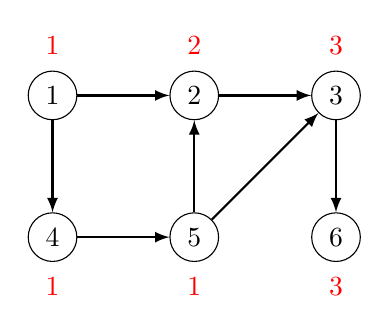
\begin{tikzpicture}[scale=0.9]
\node[draw, circle] (1) at (1,5) {$1$};
\node[draw, circle] (2) at (3,5) {$2$};
\node[draw, circle] (3) at (5,5) {$3$};
\node[draw, circle] (4) at (1,3) {$4$};
\node[draw, circle] (5) at (3,3) {$5$};
\node[draw, circle] (6) at (5,3) {$6$};

\path[draw,thick,->,>=latex] (1) -- (2);
\path[draw,thick,->,>=latex] (2) -- (3);
\path[draw,thick,->,>=latex] (1) -- (4);
\path[draw,thick,->,>=latex] (4) -- (5);
\path[draw,thick,->,>=latex] (5) -- (2);
\path[draw,thick,->,>=latex] (5) -- (3);
\path[draw,thick,->,>=latex] (3) -- (6);

\node[color=red] at (1,2.3) {$1$};
\node[color=red] at (3,2.3) {$1$};
\node[color=red] at (5,2.3) {$3$};
\node[color=red] at (1,5.7) {$1$};
\node[color=red] at (3,5.7) {$2$};
\node[color=red] at (5,5.7) {$3$};
\end{tikzpicture}
\end{center}

Na primjer, za izračun vrijednosti $\texttt{paths}(3)$
možemo koristiti formulu $\texttt{paths}(2)+\texttt{paths}(5)$,
jer postoje bridovi iz čvorova 2 i 5
do čvora 3.
Budući da je $\texttt{paths}(2)=2$ i $\texttt{paths}(5)=1$, zaključujemo da je $\texttt{paths}(3)=3$.

\subsubsection{Proširenje Dijkstrinog algoritma}

\index{Dijkstrin algoritam}

Nusproizvod Dijkstrinog algoritma je usmjereni, aciklički
graf koji za svaki čvor izvornog grafa pokazuje
moguće načine na koje se do tog čvora može doći najkraćim putem
iz početnog čvora.
Na taj se graf može primijeniti dinamičko programiranje.
Na primjer, u grafu
\begin{center}
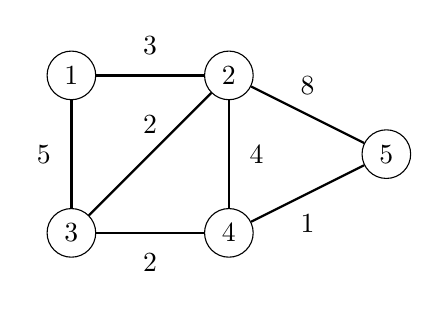
\begin{tikzpicture}
\node[draw, circle] (1) at (0,0) {$1$};
\node[draw, circle] (2) at (2,0) {$2$};
\node[draw, circle] (3) at (0,-2) {$3$};
\node[draw, circle] (4) at (2,-2) {$4$};
\node[draw, circle] (5) at (4,-1) {$5$};

\path[draw,thick,-] (1) -- node[font=\small,label=above:3] {} (2);
\path[draw,thick,-] (1) -- node[font=\small,label=left:5] {} (3);
\path[draw,thick,-] (2) -- node[font=\small,label=right:4] {} (4);
\path[draw,thick,-] (2) -- node[font=\small,label=above:8] {} (5);
\path[draw,thick,-] (3) -- node[font=\small,label=below:2] {} (4);
\path[draw,thick,-] (4) -- node[font=\small,label=below:1] {} (5);
\path[draw,thick,-] (2) -- node[font=\small,label=above:2] {} (3);
\end{tikzpicture}
\end{center}
najkraći putovi iz čvora 1 mogu koristiti sljedeće bridove:
\begin{center}
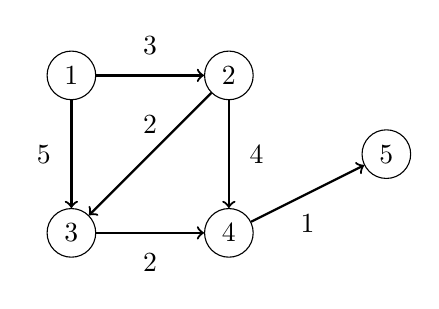
\begin{tikzpicture}
\node[draw, circle] (1) at (0,0) {$1$};
\node[draw, circle] (2) at (2,0) {$2$};
\node[draw, circle] (3) at (0,-2) {$3$};
\node[draw, circle] (4) at (2,-2) {$4$};
\node[draw, circle] (5) at (4,-1) {$5$};

\path[draw,thick,->] (1) -- node[font=\small,label=above:3] {} (2);
\path[draw,thick,->] (1) -- node[font=\small,label=left:5] {} (3);
\path[draw,thick,->] (2) -- node[font=\small,label=right:4] {} (4);
\path[draw,thick,->] (3) -- node[font=\small,label=below:2] {} (4);
\path[draw,thick,->] (4) -- node[font=\small,label=below:1] {} (5);
\path[draw,thick,->] (2) -- node[font=\small,label=above:2] {} (3);
\end{tikzpicture}
\end{center}

Sada možemo, na primjer, dinamičkim programiranjem
izračunati broj najkraćih putova
od čvora 1 do čvora 5:
\begin{center}
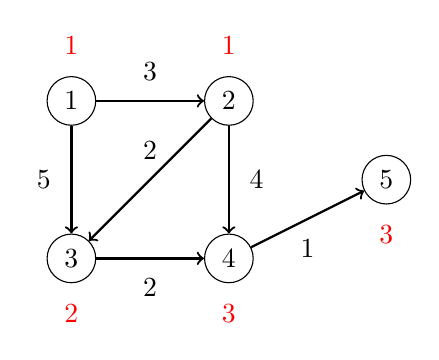
\begin{tikzpicture}
\node[draw, circle] (1) at (0,0) {$1$};
\node[draw, circle] (2) at (2,0) {$2$};
\node[draw, circle] (3) at (0,-2) {$3$};
\node[draw, circle] (4) at (2,-2) {$4$};
\node[draw, circle] (5) at (4,-1) {$5$};

\path[draw,thick,->] (1) -- node[font=\small,label=above:3] {} (2);
\path[draw,thick,->] (1) -- node[font=\small,label=left:5] {} (3);
\path[draw,thick,->] (2) -- node[font=\small,label=right:4] {} (4);
\path[draw,thick,->] (3) -- node[font=\small,label=below:2] {} (4);
\path[draw,thick,->] (4) -- node[font=\small,label=below:1] {} (5);
\path[draw,thick,->] (2) -- node[font=\small,label=above:2] {} (3);

\node[color=red] at (0,0.7) {$1$};
\node[color=red] at (2,0.7) {$1$};
\node[color=red] at (0,-2.7) {$2$};
\node[color=red] at (2,-2.7) {$3$};
\node[color=red] at (4,-1.7) {$3$};
\end{tikzpicture}
\end{center}

\subsubsection{Prikaz zadataka pomoću grafova}

Zapravo se svaki zadatak dinamičkog programiranja
može prikazati kao usmjereni, aciklički graf.
U takvom grafu svaki čvor odgovara jednom stanju dinamičkog programiranja,
a bridovi pokazuju kako stanja ovise jedno o drugome.

Kao primjer, razmotrimo zadatak
sastavljanja svote novca $n$
pomoću kovanica
$\{c_1,c_2,\ldots,c_k\}$.
U tom zadatku možemo konstruirati graf u kojem
svaki čvor odgovara jednoj svoti novca,
a bridovi pokazuju kako se kovanice mogu odabrati.
Na primjer, za kovanice $\{1,3,4\}$ i $n=6$
graf izgleda ovako:
\begin{center}
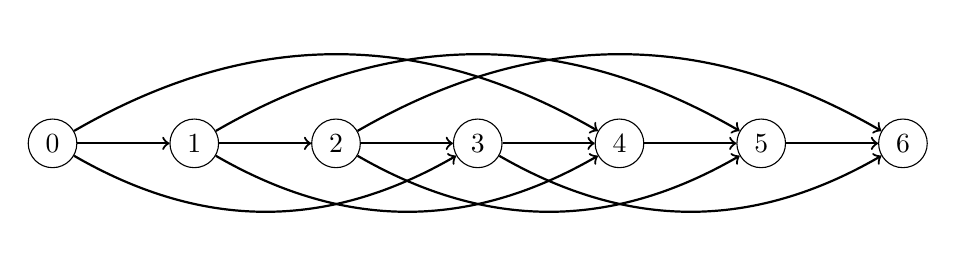
\begin{tikzpicture}[scale=0.9]
\node[draw, circle] (0) at (0,0) {$0$};
\node[draw, circle] (1) at (2,0) {$1$};
\node[draw, circle] (2) at (4,0) {$2$};
\node[draw, circle] (3) at (6,0) {$3$};
\node[draw, circle] (4) at (8,0) {$4$};
\node[draw, circle] (5) at (10,0) {$5$};
\node[draw, circle] (6) at (12,0) {$6$};

\path[draw,thick,->] (0) -- (1);
\path[draw,thick,->] (1) -- (2);
\path[draw,thick,->] (2) -- (3);
\path[draw,thick,->] (3) -- (4);
\path[draw,thick,->] (4) -- (5);
\path[draw,thick,->] (5) -- (6);

\path[draw,thick,->] (0) edge [bend right=30] (3);
\path[draw,thick,->] (1) edge [bend right=30] (4);
\path[draw,thick,->] (2) edge [bend right=30] (5);
\path[draw,thick,->] (3) edge [bend right=30] (6);

\path[draw,thick,->] (0) edge [bend left=30] (4);
\path[draw,thick,->] (1) edge [bend left=30] (5);
\path[draw,thick,->] (2) edge [bend left=30] (6);
\end{tikzpicture}
\end{center}

Uz takav prikaz
najkraći put od čvora 0 do čvora $n$
odgovara rješenju s najmanjim brojem kovanica,
a ukupan broj putova od čvora 0 do čvora $n$
jednak je ukupnom broju rješenja.

\section{Putovi sljedbenika}

\index{graf sljedbenika}
\index{funkcijski graf}

U ostatku poglavlja
usredotočit ćemo se na \key{grafove sljedbenika}.
U tim grafovima
izlazni stupanj svakog čvora je 1, tj.
iz svakog čvora izlazi točno jedan brid.
Graf sljedbenika sastoji se od jedne ili više
komponenti, od kojih svaka sadrži
jedan ciklus i nekoliko putova koji vode do njega.

Grafovi sljedbenika se ponekad nazivaju
\key{funkcijski grafovi}.
Razlog je to što svaki graf sljedbenika
odgovara funkciji koja definira
bridove grafa.
Parametar te funkcije je čvor grafa,
a funkcija daje sljedbenika toga čvora.

Na primjer, funkcija
\begin{center}
\begin{tabular}{r|rrrrrrrrr}
$x$ & 1 & 2 & 3 & 4 & 5 & 6 & 7 & 8 & 9 \\
\hline
$\texttt{succ}(x)$ & 3 & 5 & 7 & 6 & 2 & 2 & 1 & 6 & 3 \\
\end{tabular}
\end{center}
definira sljedeći graf:
\begin{center}
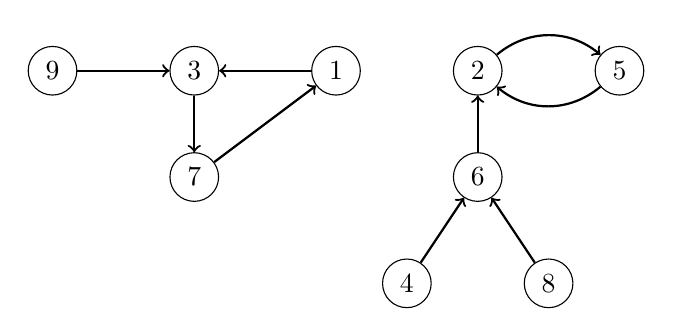
\begin{tikzpicture}[scale=0.9]
\node[draw, circle] (1) at (0,0) {$1$};
\node[draw, circle] (2) at (2,0) {$2$};
\node[draw, circle] (3) at (-2,0) {$3$};
\node[draw, circle] (4) at (1,-3) {$4$};
\node[draw, circle] (5) at (4,0) {$5$};
\node[draw, circle] (6) at (2,-1.5) {$6$};
\node[draw, circle] (7) at (-2,-1.5) {$7$};
\node[draw, circle] (8) at (3,-3) {$8$};
\node[draw, circle] (9) at (-4,0) {$9$};

\path[draw,thick,->] (1) -- (3);
\path[draw,thick,->] (2)  edge [bend left=40] (5);
\path[draw,thick,->] (3) -- (7);
\path[draw,thick,->] (4) -- (6);
\path[draw,thick,->] (5)  edge [bend left=40] (2);
\path[draw,thick,->] (6) -- (2);
\path[draw,thick,->] (7) -- (1);
\path[draw,thick,->] (8) -- (6);
\path[draw,thick,->] (9) -- (3);
\end{tikzpicture}
\end{center}

Budući da svaki čvor grafa sljedbenika ima
jedinstvenog sljedbenika, možemo definirati i funkciju $\texttt{succ}(x,k)$
koja daje čvor do kojega ćemo doći ako
krenemo iz čvora $x$ i prijeđemo $k$ koraka naprijed.
Na primjer, u gornjem grafu je $\texttt{succ}(4,6)=2$,
jer ćemo doći do čvora 2 prelaskom 6 koraka iz čvora 4:

\begin{center}
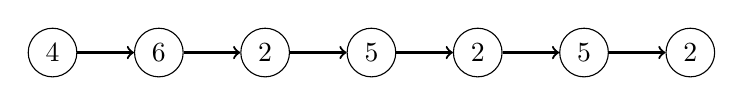
\begin{tikzpicture}[scale=0.9]
\node[draw, circle] (1) at (0,0) {$4$};
\node[draw, circle] (2) at (1.5,0) {$6$};
\node[draw, circle] (3) at (3,0) {$2$};
\node[draw, circle] (4) at (4.5,0) {$5$};
\node[draw, circle] (5) at (6,0) {$2$};
\node[draw, circle] (6) at (7.5,0) {$5$};
\node[draw, circle] (7) at (9,0) {$2$};

\path[draw,thick,->] (1) -- (2);
\path[draw,thick,->] (2) -- (3);
\path[draw,thick,->] (3) -- (4);
\path[draw,thick,->] (4) -- (5);
\path[draw,thick,->] (5) -- (6);
\path[draw,thick,->] (6) -- (7);
\end{tikzpicture}
\end{center}

Izravan način izračuna vrijednosti $\texttt{succ}(x,k)$
jest krenuti iz čvora $x$ i prijeći $k$ koraka naprijed, što traje $O(k)$ vremena.
Međutim, uz predobradu se svaka vrijednost $\texttt{succ}(x,k)$
može izračunati u samo $O(\log k)$ vremena.

Ideja je unaprijed izračunati sve vrijednosti $\texttt{succ}(x,k)$ gdje je
$k$ potencija broja dva i najviše $u$, pri čemu je $u$
najveći broj koraka koje ćemo ikada prijeći.
To se može učiniti efikasno, jer
možemo koristiti sljedeću rekurziju:

\begin{equation*}
    \texttt{succ}(x,k) = \begin{cases}
               \texttt{succ}(x)              & k = 1\\
               \texttt{succ}(\texttt{succ}(x,k/2),k/2)   & k > 1\\
           \end{cases}
\end{equation*}

Prethodni izračun vrijednosti traje $O(n \log u)$ vremena,
jer se za svaki čvor izračuna $O(\log u)$ vrijednosti.
U gornjem grafu prve vrijednosti su sljedeće:

\begin{center}
\begin{tabular}{r|rrrrrrrrr}
$x$ & 1 & 2 & 3 & 4 & 5 & 6 & 7 & 8 & 9 \\
\hline
$\texttt{succ}(x,1)$ & 3 & 5 & 7 & 6 & 2 & 2 & 1 & 6 & 3 \\
$\texttt{succ}(x,2)$ & 7 & 2 & 1 & 2 & 5 & 5 & 3 & 2 & 7 \\
$\texttt{succ}(x,4)$ & 3 & 2 & 7 & 2 & 5 & 5 & 1 & 2 & 3 \\
$\texttt{succ}(x,8)$ & 7 & 2 & 1 & 2 & 5 & 5 & 3 & 2 & 7 \\
$\cdots$ \\
\end{tabular}
\end{center}

Nakon toga se svaka vrijednost $\texttt{succ}(x,k)$ može izračunati
prikazom broja koraka $k$ kao sume potencija broja dva.
Na primjer, ako želimo izračunati vrijednost $\texttt{succ}(x,11)$,
najprije oblikujemo prikaz $11=8+2+1$.
Koristeći to,
\[\texttt{succ}(x,11)=\texttt{succ}(\texttt{succ}(\texttt{succ}(x,8),2),1).\]
Na primjer, u prethodnom grafu
\[\texttt{succ}(4,11)=\texttt{succ}(\texttt{succ}(\texttt{succ}(4,8),2),1)=5.\]

Takav prikaz uvijek se sastoji od
$O(\log k)$ dijelova, pa izračun vrijednosti $\texttt{succ}(x,k)$
traje $O(\log k)$ vremena.

\section{Otkrivanje ciklusa}

\index{ciklus}
\index{otkrivanje ciklusa}

Razmotrimo graf sljedbenika koji sadrži samo
put koji završava u ciklusu.
Možemo postaviti sljedeća pitanja:
ako započnemo šetnju u početnom čvoru,
koji je prvi čvor u ciklusu
i koliko čvorova ciklus sadrži?

Na primjer, u grafu

\begin{center}
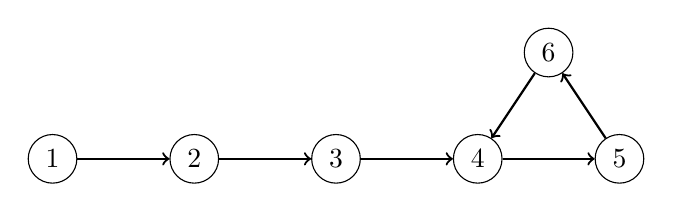
\begin{tikzpicture}[scale=0.9]
\node[draw, circle] (5) at (0,0) {$5$};
\node[draw, circle] (4) at (-2,0) {$4$};
\node[draw, circle] (6) at (-1,1.5) {$6$};
\node[draw, circle] (3) at (-4,0) {$3$};
\node[draw, circle] (2) at (-6,0) {$2$};
\node[draw, circle] (1) at (-8,0) {$1$};

\path[draw,thick,->] (1) -- (2);
\path[draw,thick,->] (2) -- (3);
\path[draw,thick,->] (3) -- (4);
\path[draw,thick,->] (4) -- (5);
\path[draw,thick,->] (5) -- (6);
\path[draw,thick,->] (6) -- (4);
\end{tikzpicture}
\end{center}
šetnju započinjemo u čvoru 1,
prvi čvor koji pripada ciklusu je čvor 4, a ciklus se sastoji
od tri čvora (4, 5 i 6).

Jednostavan način otkrivanja ciklusa jest šetati po
grafu i pratiti
sve čvorove koji su posjećeni. Kada je neki čvor posjećen
drugi put, možemo zaključiti
da je taj čvor prvi čvor u ciklusu.
Ova metoda radi u $O(n)$ vremena i također koristi
$O(n)$ memorije.

Međutim, postoje bolji algoritmi za otkrivanje ciklusa.
Vremenska složenost takvih algoritama je i dalje $O(n)$,
ali oni koriste samo $O(1)$ memorije.
To je važno poboljšanje ako je $n$ velik.
Sljedeće ćemo razmotriti Floydov algoritam koji
ostvaruje ta svojstva.

\subsubsection{Floydov algoritam}

\index{Floydov algoritam}

\key{Floydov algoritam}\footnote{Ideja algoritma spominje se u \cite{knu982}
i pripisuje se R. W. Floydu; međutim, nije poznato je li Floyd zaista
otkrio taj algoritam.} šeta naprijed
po grafu koristeći dva pokazivača $a$ i $b$.
Oba pokazivača počinju u čvoru $x$ koji
je početni čvor grafa.
Zatim, u svakom koraku, pokazivač $a$ prelazi
jedan korak naprijed, a pokazivač $b$
prelazi dva koraka naprijed.
Postupak se nastavlja dok se
pokazivači ne susretnu:
\begin{lstlisting}
a = succ(x);
b = succ(succ(x));
while (a != b) {
    a = succ(a);
    b = succ(succ(b));
}
\end{lstlisting}

U tom trenutku pokazivač $a$ je prešao $k$ koraka,
a pokazivač $b$ je prešao $2k$ koraka,
pa duljina ciklusa dijeli $k$.
Stoga se prvi čvor koji pripada ciklusu
može naći premještanjem pokazivača $a$ u čvor $x$
i pomicanjem pokazivača
korak po korak dok se ponovno ne susretnu.
\begin{lstlisting}
a = x;
while (a != b) {
    a = succ(a);
    b = succ(b);
}
first = a;
\end{lstlisting}

Nakon toga se duljina ciklusa
može izračunati na sljedeći način:
\begin{lstlisting}
b = succ(a);
length = 1;
while (a != b) {
    b = succ(b);
    length++;
}
\end{lstlisting}
